
%(BEGIN_QUESTION)
% Copyright 2007, Tony R. Kuphaldt, released under the Creative Commons Attribution License (v 1.0)
% This means you may do almost anything with this work of mine, so long as you give me proper credit

The following differential pressure sensor uses a matched pair of strain gauges.  As the differential pressure increases, one strain gauge becomes compressed while the other becomes stretched.  A voltmeter registers the bridge circuit's imbalance and displays it as a pressure measurement:

$$\includegraphics[width=15.5cm]{i02944x01.eps}$$

\vskip 10pt

\noindent
Determine the following:

\begin{itemize}
\item{} Identify which port is the ``high'' pressure port
\item{} Identify what the voltmeter will register if fixed resistor $R_1$ fails open
\item{} Identify a component fault that would drive the voltmeter full upscale (``peg'' positive)
\item{} Identify another component fault that would drive the voltmeter full upscale (``peg'' positive)
\end{itemize}

\underbar{file i02944}
%(END_QUESTION)





%(BEGIN_ANSWER)

\begin{itemize}
\item{} Which port is the ``high'' pressure port: {\bf Port ``B''}
\item{} What will happen if fixed resistor $R_1$ fails open: {\bf Voltmeter will drive fully upscale (``peg'' positive)}
\item{} Identify a component fault that would drive the voltmeter full upscale (``peg'' positive):
\item\item{} Strain gauge \#1 fails shorted
\item\item{} Strain gauge \#2 fails open
\item\item{} $R_1$ fails open
\item\item{} $R_2$ fails shorted
\end{itemize}

%(END_ANSWER)





%(BEGIN_NOTES)

\vskip 20pt \vbox{\hrule \hbox{\strut \vrule{} {\bf Virtual Troubleshooting} \vrule} \hrule}

This question is a good candidate for a ``Virtual Troubleshooting'' exercise.  Presenting the diagram to students, you first imagine in your own mind a particular fault in the system.  Then, you present one or more symptoms of that fault (something noticeable by an operator or other user of the system).  Students then propose various diagnostic tests to perform on this system to identify the nature and location of the fault, as though they were technicians trying to troubleshoot the problem.  Your job is to tell them what the result(s) would be for each of the proposed diagnostic tests, documenting those results where all the students can see.

During and after the exercise, it is good to ask students follow-up questions such as:

\begin{itemize}
\item{} What does the result of the last diagnostic test tell you about the fault?
\item{} Suppose the results of the last diagnostic test were different.  What then would that result tell you about the fault?
\item{} Is the last diagnostic test the best one we could do?
\item{} What would be the ideal order of tests, to diagnose the problem in as few steps as possible?
\end{itemize}


%INDEX% Measurement, pressure: ``high'' versus ``low'' ports of a DP instrument
%INDEX% Troubleshooting review: electric circuits

%(END_NOTES)


